\subsection{Hidden Markov Models}

HMMs are common statistical models used to describe time series that exhibit state-switching behavior. An HMM models an observed sequence of length $T$, $\bfY = \{Y_t\}_{t=1}^T$, together with an unobserved (or  ``hidden") sequence $\bfX = \{X_t\}_{t=1}^T$. The hidden sequence $\bfX$ is a Markov chain, and each observation $Y_t$ is a random variable, where $Y_t$ given all other observations $\bfY \setminus \{Y_t\}$ and hidden states $\bfX$ depends only on $X_t$. While the sample space of $\bfX$ is general, we assume $X_t \in \{1,\ldots,N\}$ for some finite $N$. The unconditional distribution of $X_1$ is denoted by the row-vector
%
%\begin{equation}
$\bfdelta = \begin{pmatrix} \delta_{1} & \cdots & \delta_{N} \end{pmatrix}$,
%\end{equation}
%
where $\delta_{i} = \bbP(X_1 = i)$. Further, the distribution of $X_t$ for $t > 1$ conditioned on $X_{t-1}$ is denoted by an $N$-by-$N$ transition probability matrix
%
\begin{equation}
    \bfGamma_t = \begin{pmatrix} 
    \Gamma_{t,1,1} & \cdots & \Gamma_{t,1,N} \\
    \vdots & \ddots & \vdots \\
    \Gamma_{t,N,1} & \cdots & \Gamma_{t,N,N} \\
    \end{pmatrix},
\end{equation}
%
where $\Gamma_{t,i,j} = \bbP(X_t = j \mid X_{t-1} = i)$. %Our methods apply to transition probability matrices that depend upon time, but for ease of presentation
For simplicity, we assume that $\bfGamma_t$ does not change over time (i.e. $\bfGamma_t = \bfGamma$ for all $t$) unless stated otherwise. 
%
%We assume that the distribution of an observation $Y_t$ conditioned on the corresponding hidden state $X_t$ does not depend upon any other observation or hidden state.
%Some variants of HMMs allow $Y_t$ to depend upon both $Y_{t-1}$ and $X_t$. Our methodology can be straightforwardly applied to such HMMs, but for clarity of presentation we assume that $Y_t$ depends only on $X_t$. 
%
To ensure that all entries are positive and all rows sum to one, it is convenient to reparameterize the transition probability matrix $\bfGamma$ and initial distribution $\bfdelta \in \bbR^N$ in terms of an auxiliary variable $\bfeta$: %follow the parameterization of \citet{Barajas:2017}:
%
\begin{equation}
    \Gamma_{i,j}(\bfeta) = \frac{\exp(\eta_{i,j})}{\sum_{j'=1}^N \exp(\eta_{i,j'})}, \qquad \delta_{i}(\bfeta) = \frac{\exp(\eta_{i})}{\sum_{i'=1}^N \exp(\eta_{i'})},
    \label{eqn:reparam}
\end{equation}
%
where $i,j = 1,\ldots,N$ and $\eta_{i,i}$ and $\eta_{1}$ are set to zero for identifiability. This formulation simplifies likelihood maximization by removing constraints in the optimization problem. One may also incorporate covariates into $\bfGamma$ by setting $\eta_{i,j}(\bfz_t ; \bfbeta_{i,j}) = \left(\bfbeta_{i,j}\right)^{\top} \bfz_t$, where $\bfz_t$ is a column vector of known covariates at time index $t$ and $\bfbeta_{i,j}$ is a column vector of unknown regression coefficients. While $\bfGamma$ and $\bfdelta$ are functions of $\bfeta$, we abuse notation in future sections and treat $\bfGamma$ and $\bfdelta$ as variables since the mapping is a bijection.

If $X_t=i$, then we denote the conditional density or probability mass function of $Y_t$ as $f_{i}(\cdot ; \theta_{i})$, where $\theta_{i}$ are the parameters describing the state-dependent distribution of $Y_t$. The collection of all state-dependent parameters is $\bftheta = \{\theta_{i}\}_{i=1}^N$. For brevity, we denote the full set of parameters as $\bfphi \equiv \{\bftheta,\bfeta\}$. Figure \ref{fig:HMM} shows an HMM as a graphical model.
%
\begin{figure}[h]
    \centering
    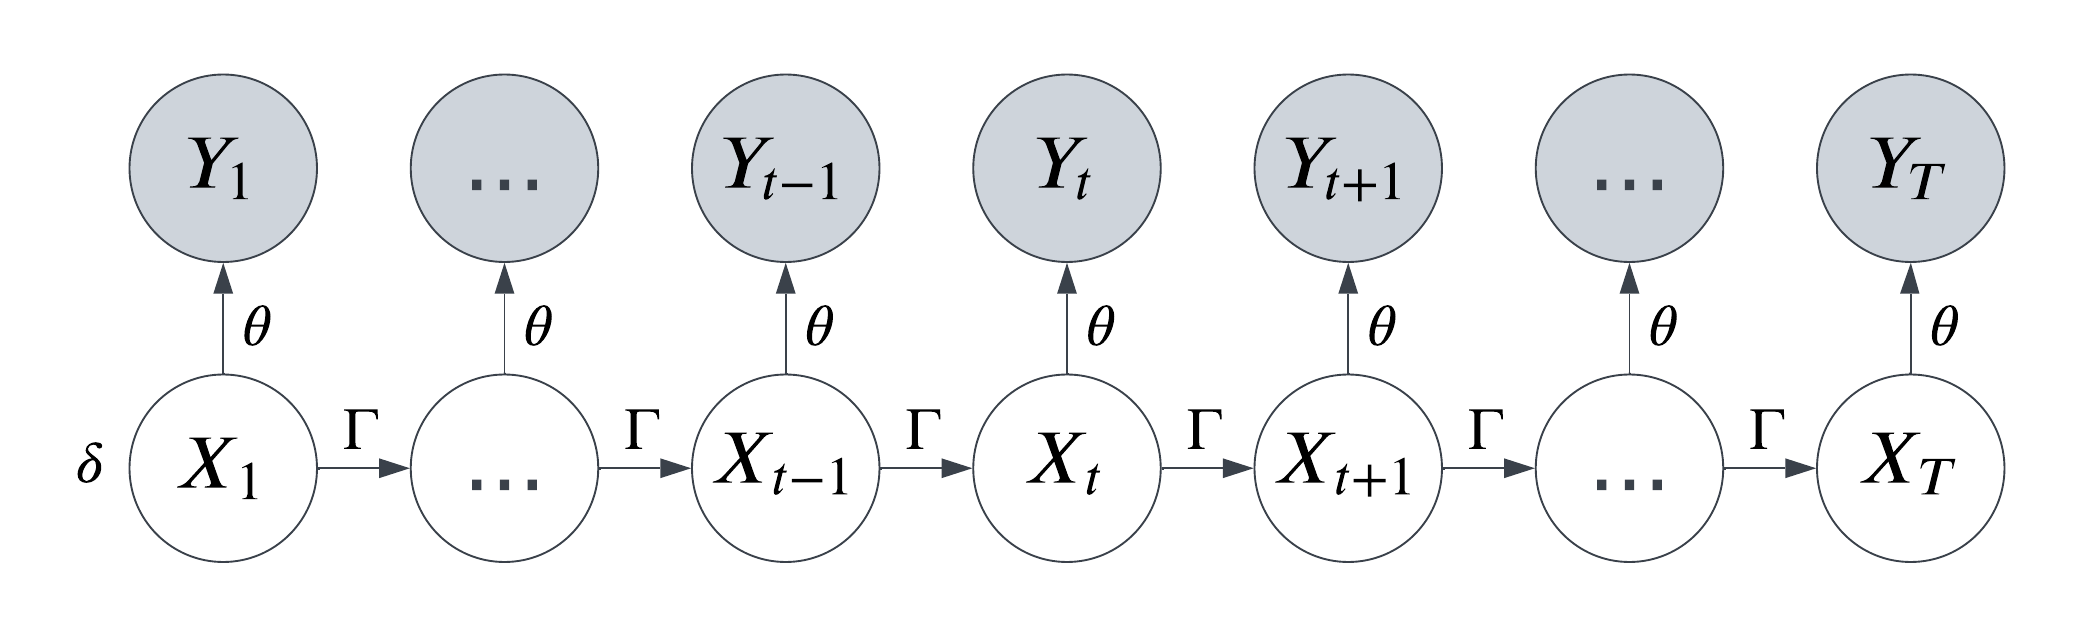
\includegraphics[width=5in]{../plt/HMM.png}
    \caption{Graphical representation of an HMM. $X_t$ corresponds to an unobserved latent state at time $t$ whose distribution is described by a Markov chain. $Y_t$ corresponds to an observation at time $t$, where $Y_t$ given all other observations $\bfY \setminus \{Y_t\}$ and hidden states $\bfX$ depends only on $X_t$.}
    \label{fig:HMM}
\end{figure}
%
%We also denote the set of parameters associated with the initial distribution as $\bfeta^{(\cdot)} = \{\eta_{i}\}_{i=1}^N$, and the set of parameters associated with the transition probability matrix as $\bfeta^{(\cdot,\cdot)} = \{\eta_{i,j}\}_{i,j=1}^N$. 

The joint likelihood of an HMM given observations $\bfY$ and latent states $\bfX$ is
%
\begin{equation}
    p(\bfX,\bfY;\bfphi) = \delta_{X_1} f_{X_1}(Y_1; \theta_{X_1}) \prod_{t=2}^T \Gamma_{X_{t-1},X_t} ~ f_{X_t}(Y_t ; \theta_{X_t}).
    \label{eqn:like}
\end{equation}
%
Alternatively, the marginal likelihood of the observed data $\bfY$ alone is 
%
\begin{equation}
    p(\bfY;\bfphi) = \bfdelta P(Y_1;\bftheta) \prod_{t=2}^T \bfGamma P(Y_t;\bftheta) \mathbf{1}^\top_N,
    \label{eqn:like_marginal}
\end{equation}
%
where $\mathbf{1}_N$ is an $N$-dimensional row vector of ones and $P(y_t;\bftheta)$ is an $N \times N$ diagonal matrix with entry $(i,i)$ equal to $f_{i}(y_t; \theta_{i})$. For a more complete introduction to HMMs, see \citet{Zucchini:2016}.
%
\subsection{State Decoding}
%
%GET RID OF TILDE FUNCTIONS IN BACKGROUND SECTION
%
%ADD FUNCTIONS (TILDES) RIGHT BEFORE ALG 4 AND MAKE TILDE FUNCTION ARGUMENTS NOT ALPHA t-1, and then comment that putting in $\alpha_t-1(\bfphi)$ gives the right value
%
%SAY THAT WE ASSUME PHI IS FIXED
%
%CHANGE GRADIENT ESTIMATES TO GRADIENT APPROXIMATIONS???
%
%ADD HATS TO ALPHAS, BETAS, ETC
%
%CHANGE WORDING FOR GRADIENTS TO APPROXIMATIONS
%
% MAKE ALL PARAMETERS BOLDED
%

One appealing feature of HMMs is that it is simple to determine the distribution of a given hidden state ($X_t$) conditioned on the set of observations $\bfY$. Assuming that the HMM parameters $\bfphi$ are fixed, define the probability density of the observations between times $s$ and $t$ as $p(Y_{s:t};\bfphi)$. Likewise, define \textit{forward probabilities} $\alpha_{t,i} = p(y_{1:t},X_t = i;\bfphi)$ (for $i = 1,\ldots,N$ and $t = 1,\ldots,T$) and \textit{backward probabilities} $\beta_{t,i} = p(y_{(t+1):T}|X_t = i;\bfphi)$ (for $i = 1,\ldots,N$ and $t = 1,\ldots,T-1$). By convention, $\beta_{T,i} = 1$ for $i = 1,\ldots,N$. We thus define the row vectors $\bfalpha_t = \begin{pmatrix} \alpha_{t,1} & \cdots & \alpha_{t,N} \end{pmatrix}$ and $\bfbeta_t = \begin{pmatrix} \beta_{t,1} & \cdots & \beta_{t,N} \end{pmatrix}$. Both $\bfalpha_t$ and $\bfbeta_t$ can be calculated using the following recursions: % We define the mapping from $\alpha_{t-1}(\bfphi)$ and $\bfphi$ to $\alpha_t(\bfphi)$ as $\tilde \alpha_t(\alpha_{t-1}(\bfphi),\bfphi)$. However, $\alpha_t(\bfphi)$ itself is a function of $\bfphi$ alone, which we denote as $\alpha_t$. Similarly, we define the mapping from $\beta_{t+1}(\bfphi)$ and $\bfphi$ to $\beta_{t}(\bfphi)$ as $\tilde \beta_t(\alpha_{t+1}(\bfphi),\bfphi)$ and the mapping from only $\bfphi$ to $\beta_t$ as $\beta_t(\bfphi)$. 

\begin{gather}
    \bfalpha_1 = \bfdelta ~ P(y_1;\bftheta), \qquad 
    %
    \bfalpha_t = \bfalpha_{t-1} ~ \bfGamma ~ P(y_t;\bftheta), \quad t = 2,\ldots,T, \label{eqn:alpha} \\
    %
    \bfbeta^\top_T = \mathbf{1}_N^\top, \qquad
    %
    \bfbeta^\top_t = \bfGamma ~ P(y_{t+1};\bftheta) ~ \bfbeta^\top_{t+1}, \quad t = 1,\ldots,T-1. \label{eqn:beta}
\end{gather}
%It is important to note that $\alpha_t$ and $\beta_t$ are functions of $\bfphi$ alone. We nonetheless abuse notation and write $\alpha_t$ and $\beta_t$ as functions of $\alpha_{t-1}$ and $\beta_{t+1}$ as well to illustrate the recursion. In addition, it takes $\calO(N^2)$ time to calculate $\alpha_{t}$ and $\beta_{t}$ if $\alpha_{t-1}$, $\beta_{t+1}$, and $\bfphi$ are known. However, it takes $\calO(TN^2)$ time to calculate $\alpha_{t}$ and $\beta_{t}$ if only $\bfphi$ is known, as the recursions starting from $\alpha_1$ and $\beta_T$ must be performed.
%
%Note that it takes $\calO(N^2)$ time to evaluate $\tilde \alpha_t (\alpha_{t-1},\bfphi)$ and $\tilde \beta_t(\beta_{t+1},\bfphi)$, but $\calO(TN^2)$ time to evaluate $\alpha_t(\bfphi)$ and $\beta_t(\bfphi)$. 
%In future sections we abuse notation and write $\alpha_t(\bfphi)$ and $\beta_t(\bfphi)$ as $\alpha_t$ and $\beta_t$ for brevity. 
%We denote the probability that $X_t = i$ given all observations $\bfY$ and parameters $\bfphi$ as $\gamma_{t,i}$ for $t = 1,\ldots,T$ and $i = 1,\ldots,N$. Further, we denote the probability that $X_{t-1} = i$ and $X_t = j$ given all observations $\bfY$ and parameters $\bfphi$ as $\xi_{t,i,j}$ for $t = 2,\ldots,T$ and $i,j = 1,\ldots,N$. Namely,
We define conditional probabilities $\gamma_{t,i} = \bbP(X_t = i \mid \bfY ~;~ \bfphi)$ and $\xi_{t,i,j} = \bbP(X_{t-1} = i, X_t = j \mid \bfY ~;~ \bfphi)$.
%
%\begin{gather}
%    \gamma_{t,i} = \bbP(X_t = i \mid \bfY ~;~ \bfphi), \label{eqn:gamma_prob} \\ 
    %
%    \xi_{t,i,j} = \bbP(X_{t-1} = i, X_t = j \mid \bfY ~;~ \bfphi). \label{eqn:xi_prob}
%\end{gather}
%
Further, define the row vector $\bfgamma_t = \begin{pmatrix} \gamma_{t,1} & \cdots & \gamma_{t,N} \end{pmatrix}$ and the matrix 

\begin{equation*}
    \bfxi_t = \begin{pmatrix} 
    \xi_{t,1,1} & \cdots & \xi_{t,1,N} \\
    \vdots & \ddots & \vdots \\
    \xi_{t,N,1} & \cdots & \xi_{t,N,N} \\
    \end{pmatrix}, \qquad t = 2,\ldots,T. 
\end{equation*}
%
Both $\bfgamma_t$ and $\bfxi_t$ can be calculated from $\bfalpha_{t-1}$, $\bfalpha_t$, $\bfbeta_t$, $\bfGamma$, and $\bftheta$ as follows. Let $\text{diag}(\cdot)$ map a row vector to the diagonal matrix with that row vector as its diagonal. Then,

\begin{gather}
    \gamma_{t,i} = \frac{\alpha_{t,i} ~ \beta_{t,i}}{\bfalpha_{t} ~ \bfbeta_t^\top}, \qquad \bfgamma_t = \frac{\bfalpha_t ~ \text{diag}(\bfbeta_t)}{\bfalpha_t ~ \bfbeta_t^\top} \label{eqn:gamma}, \\
    %
    \xi_{t,i,j} = \frac{\alpha_{t-1,i} ~ \Gamma_{i,j} ~ f_{j}(y_{t};\theta_{j}) ~ \beta_{t,j}}{\bfalpha_{t-1} ~ \bfGamma ~ P(y_{t};\bftheta) ~ \bfbeta_{t}^\top}, \qquad \bfxi_t = \frac{\text{diag}(\bfalpha_{t-1}) ~ \bfGamma ~ P(y_t;\bftheta) ~ \text{diag}(\bfbeta_t)}{\bfalpha_{t-1} ~ \bfGamma ~ P(y_{t};\bftheta) ~ \bfbeta_{t}^\top} \label{eqn:xi}.
\end{gather}
%
%It takes $\calO(N^2)$ time to evaluate $\tilde \gamma_{t}(\alpha_t,\beta_t)$ and $\tilde \xi_{t,i,j}(\alpha_{t-1},\beta_{t},\bfphi)$, but $\calO(TN^2)$ time to evaluate $\gamma_t(\bfphi)$ and $\xi_t(\bfphi)$. %In future sections we abuse notation and write $\gamma_t(\bfphi)$ and $\xi_t(\bfphi)$ as $\gamma_t$ and $\xi_t$ for brevity. 
%
In future sections, and in particular when $\bfphi$ is not fixed (e.g. during the parameter estimation procedures), we add an argument to the conditional probabilities and write $\bfalpha(\bfphi)$, $\bfbeta(\bfphi)$, $\bfgamma(\bfphi)$, and $\bfxi(\bfphi)$ to highlight how all are functions of the parameters $\bfphi$. 

\subsection{The Baum-Welch Algorithm}

The Baum-Welch algorithm is a specific instance of the EM algorithm used to estimate the parameters of the HMM. %Suppose a sequence of observations $\bfY$ is observed as output of a latent-variable model with unknown latent states $\bfX$ and unknown parameters $\bfphi$.
At iteration $k$ of the EM algorithm, denote the current parameter estimates as $\bfphi^{(k)}$. One iteration of the EM algorithm consists of an expectation (or E) step, followed by a maximization (or M) step. For the E step, the function $Q(\bfphi \mid \bfphi^{(k)})$ is defined as the expected value of the joint log-likelihood $\log p(\bfX,\bfY; \bfphi)$ taken with respect to $\bfX$, a random variable with density $p(\bfX \mid \bfY ; \bfphi^{(k)})$. For the M step, the next parameter estimate $\bfphi^{(k+1)}$ is found by maximizing $Q(\bfphi \mid \bfphi^{(k)})$ with respect to the parameters $\bfphi$:

\begin{gather}
    Q(\bfphi \mid \bfphi^{(k)}) \equiv \bbE_{\bfphi^{(k)}}\left[\log p(\bfX,\bfY;\bfphi) \mid \bfY \right] \label{eqn:Q}, \\
    %
    %Q^*(\bfphi^{(k)}) \equiv \max_{\bfphi}Q(\bfphi \mid \bfphi^{(k)})\\
    %
    \bfphi^{(k+1)} = \argmax_{\bfphi} Q(\bfphi \mid \bfphi^{(k)}). \label{eqn:BW_update}
\end{gather}
%
For notational convenience, denote the conditional probabilities $\{\bfalpha_t(\bfphi^{(k)}), \bfbeta_t(\bfphi^{(k)}), \bfgamma_t(\bfphi^{(k)}), \bfxi_t(\bfphi^{(k)})\}$ as $\{\bfalpha_t^{(k)},\bfbeta_t^{(k)},\bfgamma_t^{(k)},\bfxi_t^{(k)}\}$. 
Substituting Equation (\ref{eqn:like}) into Equation (\ref{eqn:Q}) and performing some algebra yields a closed form expression for $Q$: %separate the expected value into three convenient terms:
\begin{equation}
    Q(\bfphi \mid \bfphi^{(k)}) %&\equiv \bbE_{\bfphi^{(k)}}\left[\log p(\bfX,\bfY;\bfphi) \mid \bfY \right] \\
    %
    %&= \bbE_{\bfphi^{(k)}} \left[\sum_{t=1}^T \log f_{X_t}(y_t;\theta_{X_t}) + \log \delta_{X_1} + \sum_{t=2}^{T} \log \Gamma^{(X_{t-1},X_{t})} \mid \bfY \right] \\
    %
    %&= \sum_{t = 1}^T \bbE_{\bfphi^{(k)}} \left[ \log f_{X_t}(y_t;\theta_{X_t}) \mid \bfY \right]  \\
    %& \qquad + \bbE_{\bfphi^{(k)}} \Big[\log \delta_{X_1} \mid \bfY \Big] + \sum_{t=2}^{T} \bbE_{\bfphi^{(k)}} \left[ \log \Gamma^{(X_{t-1},X_{t})} \mid \bfY \right] \\
    %
    = \sum_{i=1}^N \gamma_{1,i}^{(k)} \log \delta_{i}(\bfeta) + \sum_{t = 1}^T \sum_{i=1}^N \gamma_{t,i}^{(k)} \log f_{i}(y_t;\theta_{i}) + \sum_{t=2}^{T} \sum_{i=1}^N \sum_{j=1}^N \xi_{t,i,j}^{(k)} \log \Gamma_{i,j}(\bfeta).
    \label{eqn:Q_sum}
\end{equation}
%The first term and last two terms on the right-hand side of the equation above only depend upon $\theta$ and $\eta$, respectively. The maximization problem in Equation (\ref{eqn:BW_update}) can thus be divided into two separate sub-problems as follows. Note that we define the objective functions $F$ and $G$ below so that the M step of the EM algorithm is a minimization problem consistent with existing optimization literature.
%
%\begin{gather}
%    F_t^{(k)}(\bftheta) \equiv F_t(\theta, \bfphi^{(k)}) \equiv - \sum_{i=1}^N \gamma_{t,i}(\bfphi^{(k)}) \log f_{i}(y_t;\theta_{i}), \\
    %
%    F^{(k)}(\bftheta) \equiv F(\theta, \bfphi^{(k)}) \equiv \frac{1}{T} \sum_{t=1}^T F^{(k)}_t(\bftheta), \label{eqn:F} \\
    %
%    \theta^{(k+1)} = \argmin_{\theta} F^{(k)}(\bftheta), \label{eqn:EM_update_theta} \\ \nonumber \\
    %
    %
%    G_1^{(k)}(\eta) \equiv G_1(\eta, \bfphi^{(k)}) \equiv - \sum_{i=1}^N \gamma_{i}_1(\bfphi^{(k)})\log \delta_{i}(\eta) \\
    %
%    G_t^{(k)}(\eta) \equiv G_t(\eta, \bfphi^{(k)}) \equiv - \sum_{i=1}^N \sum_{j=1}^N \xi_{i,j}_t(\bfphi^{(k)}) \log \Gamma_{i,j}(\eta), \quad t \geq 2 \\
    %
%    G^{(k)}(\eta) \equiv G(\eta, \bfphi^{(k)}) = \frac{1}{T} \sum_{t=1}^{T} G_t(\eta, \bfphi^{(k)}), \label{eqn:G}\\
    %
%    \eta^{(k+1)} = \argmin_{\eta} G(\eta,\bfphi^{(k)}). \label{eqn:EM_update_eta}
%\end{gather}
%In addition, note that 
%\begin{equation}
%   Q(\bfphi \mid \bfphi^{(k)}) = -T ~ \left[F(\theta, \bfphi^{(k)}) + G(\eta, \bfphi^{(k)})\right].
%\end{equation}
%
The conditional probabilities $\gamma_{t,i}^{(k)}$ and $\xi_{t,i,j}^{(k)}$ thus act as weights for $\log \delta_{i}(\bfeta)$, $\log f_{i}(y_t;\theta_{i})$, and $\log \Gamma_{i,j}(\bfeta)$ for $i,j = 1,\ldots,N$ within $Q$. We thus refer to $\bfgamma$ and $\bfxi$ as weights in future sections. Detailed pseudocode for the E and the M step are given in Algorithms (\ref{alg:E}) and (\ref{alg:EM}) below.
%
\begin{algorithm}
\caption{\texttt{E-step}($\bfphi^{(k)}$)}\label{alg:E}
\begin{algorithmic}[1]
\Require Parameter value $\bfphi^{(k)} = \{\bftheta^{(k)},\bfeta^{(k)}\}$.
%
\State $\bfalpha_1 = \bfdelta^{(k)} ~ P(y_1;\bftheta^{(k)})$
\State $\bfbeta^\top_T = \mathbf{1}_N^\top$
\For{$t = 2,\ldots,T$}
    \State $\bfalpha_t = \bfalpha_{t-1} ~ \bfGamma^{(k)} ~ P(y_t;\bftheta^{(k)})$
    \State $\bfbeta^\top_{T-t+1} = \bfGamma^{(k)} ~ P(y_{T-t+2};\bftheta^{(k)}) ~ \bfbeta^\top_{T-t+2}$
\EndFor
%
\State $\bfgamma_1 = \frac{\bfalpha_1 ~ \text{diag}(\bfbeta_1)}{\bfalpha_1 ~ \bfbeta_1^\top}$
%
\For{$t = 2,\ldots,T$}
    \State $\bfgamma_t = \frac{\bfalpha_t ~ \text{diag}(\bfbeta_t)}{\bfalpha_t ~ \bfbeta_t^\top}$
    \State $\bfxi_t = \frac{\text{diag}(\bfalpha_{t-1}) ~ \bfGamma^{(k)} ~ P(y_t;\bftheta^{(k)}) ~ \text{diag}(\bfbeta_t)}{\bfalpha_{t-1} ~ \bfGamma^{(k)} ~ P(y_{t};\bftheta^{(k)}) ~ \bfbeta_{t}^\top}$
\EndFor
%
\State \Return $\{\bfalpha_t,\bfbeta_t,\bfgamma_t,\bfxi_t\}_{t=1}^T$
\end{algorithmic}
\end{algorithm}
%
%
%
\begin{algorithm}
\caption{\texttt{Baum-Welch}$(\bfphi^{(0)},K)$}\label{alg:EM}
\begin{algorithmic}[1]
\Require Initial parameter values $\bfphi_0$, number of iterations $K$
\For{$k = 0,\ldots,K-1$}
    \State $\{\bfalpha_{t}^{(k)},\bfbeta_{t}^{(k)},\bfgamma_{t}^{(k)},\bfxi_{t}^{(k)}\}_{t=1}^T = \texttt{E-step}(\bfphi^{(k)})$ \Comment{E step} 
    \State \Comment{M step} $$\bfphi^{(k+1)} = \argmax_{\{\bftheta,\bfeta\}} \sum_{i=1}^N \gamma_{1,i}^{(k)} \log \delta_{i}(\bfeta) + \sum_{t = 1}^T \sum_{i=1}^N \gamma_{t,i}^{(k)} \log f_{i}(y_t;\theta_{i}) + \sum_{t=2}^{T} \sum_{i=1}^N \sum_{j=1}^N \xi_{t,i,j}^{(k)} \log \Gamma_{i,j}(\bfeta)$$
\EndFor
\State \Return $\bfphi^{(K)}$
\end{algorithmic}
\end{algorithm}
%
In some simple scenarios, the maximization problem in Equation (\ref{eqn:BW_update}) above has a closed-form solution. %For example, if $\bfGamma$ does not depend upon any covariates and $f_{i}(y_t;\theta_{i})$ is a normal or Poisson probability density function with respect to $y_t$, then the solution of Equation (\ref{eqn:BW_update}) is given in Section 4.2 of \citet{Zucchini:2016}. 
However, in many cases, this maximization problem is not straightforward and requires numerical maximization techniques. %For example, finding closed-form solutions to the M step for the HHMM defined in section \ref{subsec:HHMM} is not straightforward. 
We thus review different methods for numerical maximization via stochastic optimization. %We describe several such scenarios in the subsequent section. 

\subsection{Stochastic Optimization}
\label{subsec:stoch_optim}

Stochastic optimization techniques are used to solve minimization problems where the objective function is a sum of many terms \citep{Robbins:1951}, %In much of the stochastic optimization literature, this optimization problem takes the form of a minimization over an average:
namely to solve
%
\begin{equation}
    \bfphi^* = \argmin_{\bfphi} F(\bfphi), \quad \text{where} \quad F(\bfphi) = \frac{1}{T}\sum_{t = 1}^T F_t(\bfphi).
    \label{eqn:stoch_opt}
\end{equation}
%

Standard gradient descent at a given step $m$ with step size $\lambda$ updates the parameter value $\bfphi^{(m)}$ by moving in the direction of the negative gradient of $F$. Formally, the update step is written as
%
%\begin{equation}
    $\bfphi^{(m+1)} = \bfphi^{(m)} - \lambda \nabla F(\bfphi^{(m)})$, which for our problem can be written as $\bfphi^{(m+1)} = \bfphi^{(m)} - (\lambda/T) \sum_{t=1}^T \nabla F_t(\bfphi^{(m)})$.
%\end{equation}
%
The step size $\lambda$ is a user-defined value that should be large enough to allow the algorithm to move quickly to a minimum of $F$, but not so large that $\bfphi^{(m+1)}$ ``overshoots" the minimum. This update requires evaluating a gradient for all $t = 1,\ldots,T$, which can be prohibitively expensive if $T$ is large. In contrast, stochastic gradient descent (SGD) updates $\bfphi$ using the following unbiased estimate of the full gradient \citep{Robbins:1951}:
%
%\begin{equation}
$\bfphi^{(m+1)} = \bfphi^{(m)} - \lambda \nabla F_{t}(\bfphi^{(m)}),$
%\end{equation}
%
for some $t \in \{1,\ldots,T\}$ selected uniformly at random at step $m$ of the algorithm. Stochastic gradient descent reduces the amount of time between updates by using an unbiased estimate of the gradient to update $\bfphi^{(m)}$. However, the gradient estimates themselves can have high variance, so stochastic gradient descent requires that the step size $\lambda$ decays over time to ensure convergence. In addition, SGD has slower convergence rates compared to full gradient descent \citep{Schmidt:2017}.

Variance-reduced stochastic optimization techniques such as stochastic average gradient descent (SAG) \citep{Schmidt:2017}, stochastic variance reduced gradient descent (SVRG) \citep{Johnson:2013}, and SAGA \citep{Defazio:2014} enjoy the speed of stochastic gradient descent as well as the convergence rates of full gradient descent. These algorithms involve storing gradient approximations at each gradient step $m$, $\widehat \nabla F_{t}^{(m)}$ for $t = 1,\ldots,T$, whose average approximates the full gradient $\nabla F(\bfphi^{(m)})$. The gradient approximations are updated at various stages in the optimization algorithm and are used to reduce the variance of the full gradient estimate used to update the parameters $\bfphi^{(m)}$. 
%In particular, SAG uses the update rule:
%
%\begin{equation}
%    \bfphi^{(m+1)} \gets \bfphi^{(m)} - \lambda \left[\frac{\nabla F^{(k)}_{t}(\bfphi^{(m)}) - \widehat \nabla F^{(k)}_{t}}{T} + \frac{1}{T} \sum_{t=1}^T \widehat \nabla F^{(k)}_{t} \right], \label{eqn:SAG_update}
%\end{equation}
%
%which is simply the table average with entry $t$ updated at step $m$. This update rule is intuitive, but it represents a biased estimate of the gradient $\nabla P(\bfphi^{(m)})$. This can slow down convergence and makes theoretical analysis of SAG difficult. 
For example, SVRG and SAGA update $\bfphi^{(m)}$ using an unbiased estimate of the gradient:
%
%\begin{equation}
    $\bfphi^{(m+1)} = \bfphi^{(m)} - \lambda \left[\nabla F_{t}(\bfphi^{(m)}) - \widehat \nabla F_{t}^{(m)} + \widehat \nabla F^{(m)} \right],$
    %\label{eqn:SAGA_update}
%\end{equation}
%
where
%
%\begin{equation}
    $\widehat \nabla F^{(m)} = (1/T) \sum_{t=1}^T \widehat \nabla F_{t}^{(m)}$.
    %\label{eqn:tbl_avg}
%\end{equation}
%Taking the expected value of the gradient estimate from (\ref{eqn:SAGA_update}) shows that it is unbiased:
%
%\begin{align}
%    \bbE\left[\nabla F^{(k)}_{t}(\bfphi^{(m)}) - \widehat \nabla F^{(k)}_{t} + \frac{1}{T} \sum_{t=1}^T \widehat \nabla F^{(k)}_{t} \right] &= \frac{1}{T} \sum_{t=1}^T \nabla F^{(k)}_{t}(\bfphi^{(m)}) - \frac{1}{T} \sum_{t=1}^T \widehat \nabla F^{(k)}_{t} + \frac{1}{T} \sum_{t=1}^T \widehat \nabla F^{(k)}_{t} \\
    %
%    &= \frac{1}{T} \sum_{t=1}^T \nabla F^{(k)}_{t}(\bfphi^{(m)}) = \nabla F^{(k)}(\bfphi^{(m)}).
%\end{align}
%
After updating the parameters at step $m$, SAGA simply updates the table average $\widehat \nabla F^{(m)}$ and the gradient approximation $\widehat \nabla F_{t}^{(m)}$.
%
%\begin{gather}
%    \widehat \nabla F \gets \widehat \nabla F + \frac{1}{T} \nabla F_{t}(\bfphi^{(m)}) - \frac{1}{T} \widehat \nabla F_{t}, \\
    %
%    \widehat \nabla F_{t} \gets \nabla F_{t}(\bfphi^{(m)}).
%\end{gather}
%
%After updating the table at position $t$ with the SAG/SAGA update rule, the table average $\frac{1}{T} \sum_{t=1}^T \widehat \nabla F^{(k)}_{t}$ must be updated using the previous estimate of $\widehat \nabla F^{(k)}_{t}$. 
%
%This trade-off should be considered by practitioners when deciding between the two algorithms. 
%
Algorithm (\ref{alg:VRSO}) outlines SVRG and SAGA in pseudocode. SAGA involves running the algorithm until convergence. However, the gradient approximations $\widehat \nabla F_{t}^{(m)}$ are never updated when using SVRG within Algorithm (\ref{alg:VRSO}). As such, SVRG involves repeatedly running Algorithm (\ref{alg:VRSO}) with $M$ scaling approximately with $T$ so that the table of gradient approximations remains up-to-date.

\begin{algorithm}
\caption{\texttt{VRSO}$(F,\bfphi^{(0)},\lambda,A,M)$}\label{alg:VRSO}
\begin{algorithmic}[1]
\Require Loss function $F = \frac{1}{T}\sum_{t=1}^T F_t$, initial value $\bfphi^{(0)}$, step size $\lambda$, algorithm $A \in \{\text{SVRG, SAGA}\}$, and number of iterations $M$.
%
\vspace{5pt}
\For{$t = 1,\ldots,T$} \Comment{initialize gradients and table average}
\State $\widehat \nabla F_{t}^{(0)} = \nabla F_t (\bfphi^{(0)})$
\EndFor
\State $\widehat \nabla F^{(0)} = (1/T) \sum_{t=1}^T \widehat \nabla F_{t}^{(0)}$
%
\For{$m = 0,\ldots,M-1$}:
    %
    \State Pick $t \in \{1,\ldots,T\}$ uniformly at random.
    %
    \State \Comment{update parameters}
    \begin{gather}
        \bfphi^{(m+1)} = \bfphi^{(m)} - \lambda \left[\nabla F_{t}(\bfphi^{(m)}) - \widehat \nabla F_{t}^{(m)} + \widehat \nabla F^{(m)} \right]
        \label{eqn:SAGA_update0}
    \end{gather}
    %
    \State $\widehat \nabla F_{t}^{(m+1)} = \widehat \nabla F_{t}^{(m)} \enspace$ for $t = 1,\ldots,T$ 
    %
    \Comment{update gradient approximations and average}
    %
    \If{$A$ = SAGA}:
        \begin{gather}
            \widehat \nabla F_{t}^{(m+1)} = \nabla F_{t}(\bfphi^{(m)}) \\
            \widehat \nabla F^{(m+1)} = \widehat \nabla F^{(m)} + \frac{1}{T} \left(\widehat \nabla F_{t}^{(m+1)} - \widehat \nabla F_{t}^{(m)}\right)
        \end{gather}
    \EndIf
\EndFor
\State \Return $\bfphi^{(M)}$
\end{algorithmic}
\end{algorithm}


%Whether or not Equations (\ref{eqn:EM_update_theta}) and (\ref{eqn:EM_update_eta}) have closed-form solutions, even defining $F^{(k)}$ and $G^{(k)}$ to initialize the optimization problem (the E-step) has a time cost of $\calO(T)$, which can be expensive for large $T$. 


%%%%%%%%%%%%